\documentclass[tikz,border=4pt]{standalone}
% Estilo común de los diagramas de bloques (se usa con \input en cada standalone)
\usepackage[defaultsans,scale=0.92]{lato}
\usepackage{libertinust1math}
\usepackage{xcolor,amsmath}
\usepackage{tikz}
\usetikzlibrary{positioning,arrows.meta,calc,shapes.geometric}
\usepackage{../../notacion}
\definecolor{ctrlazul}{HTML}{1E5AA8}\definecolor{ctrlnoche}{HTML}{14213D}
\definecolor{ctrlcoral}{HTML}{D1495B}\definecolor{ctrlverde}{HTML}{2A9D8F}
\definecolor{ctrlambar}{HTML}{E09F3E}\definecolor{ctrlgris}{HTML}{5C677D}
\definecolor{ctrlvioleta}{HTML}{6C4AB6}\definecolor{ctrlteal}{HTML}{0F7173}
\tikzset{
  >={Stealth[length=2.4mm]}, every node/.style={font=\small},
  bloque/.style={draw=ctrlnoche,fill=ctrlazul!7,thick,rounded corners=1.5pt,minimum height=9mm,minimum width=13mm,inner sep=4pt},
  suma/.style={draw=ctrlnoche,thick,circle,inner sep=0pt,minimum size=6mm},
  senal/.style={->,thick,draw=ctrlnoche},
  rot/.style={font=\footnotesize,text=ctrlgris},
}

\begin{document}
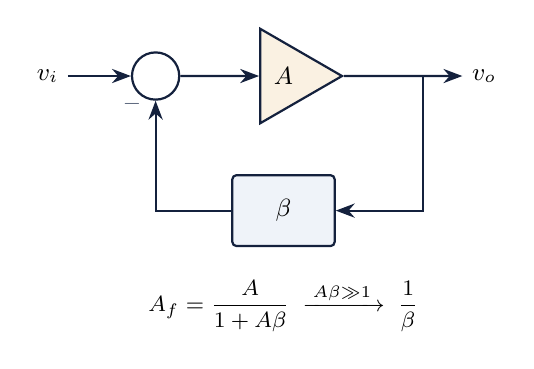
\begin{tikzpicture}[node distance=12mm]
  \node (vi) {$v_i$};
  \node[suma,right=8mm of vi] (S) {};
  \node[draw=ctrlnoche,fill=ctrlambar!15,thick,isosceles triangle,isosceles triangle apex angle=60,minimum width=12mm,right=10mm of S] (A) {$A$};
  \coordinate[right=10mm of A] (v0); \node[right=5mm of v0] (vo) {$v_o$};
  \node[bloque,below=8mm of A] (B) {$\beta$};
  \draw[senal] (vi)--(S); \draw[senal] (S)--(A); \draw[senal] (A)--(vo);
  \draw[senal] (v0) |- (B); \draw[senal] (B) -| (S); \node[rot] at ($(S)+(-3mm,-3.5mm)$) {$-$};
  \node[below=3mm of B,font=\footnotesize] {$A_f=\dfrac{A}{1+A\beta}\;\xrightarrow{\,A\beta\gg1\,}\;\dfrac1\beta$};
\end{tikzpicture}
\end{document}
